\documentclass[8pt,a4paper,landscape]{extarticle}
\makeatletter
\def\input@path{{../_shared/}}
\makeatother
\usepackage{cheatsheet}
\usepackage{graphicx}

\begin{document}
\begin{multicols*}{4}

\cheattitle{Algorithms I}{}{BA4}

% ============================================================
%                       COURSE OUTLINE
% ============================================================
% ============================================================

\section{Data Structures for Disjoint Sets}
\subsection{Disjoint sets (Union-Find)}
Each set identified by a representative.

\begin{defn}[title=Operations]
\begin{itemize}
  \item \texttt{MAKE-SET(x)}: $S_i = \{x\}$, add to $\mathcal{S}$
\end{itemize}
Let $x \in S_x$, $y \in S_y$
\begin{itemize}
  \item \texttt{UNION(x, y)}: $\mathcal{S} = \mathcal{S} \setminus \{S_x, S_y\} \cup \{S_x \cup S_y\}$
  \item \texttt{FIND(x)}: return representative of $x$ in $S_x$
\end{itemize}
\end{defn}

\begin{lstlisting}
CONNECTED-COMPONENTS(G)
    for each vertex v in G.V
        MAKE-SET(v)
    for each edge (u, v) in G.E
        if FIND(u) != FIND(v)
            UNION(u, v)
\end{lstlisting}

\subsection{Linked list representation}

\begin{center}
    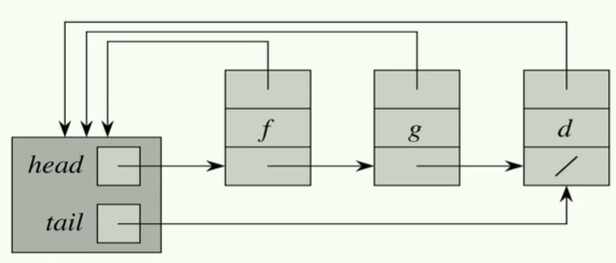
\includegraphics[width=\linewidth]{images/linkedList_representation.png}
\end{center}


\begin{thm}[title=Weighted-union heuristic]
Always merge smaller into larger. $m$ ops on $n$ elements: $O(m + n\lg n)$. Each element's representative updated $\leq \lg n$ times (each update at least doubles set size).
\end{thm}

\subsection{Tree representation}
\begin{center}
    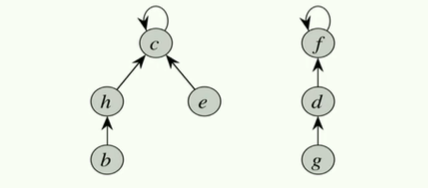
\includegraphics[width=\linewidth]{images/tree_representation.png}
\end{center}
\begin{thm}[title=Runtime with both heuristics]
\textbf{Union by rank:} smaller-rank root $\to$ child of larger-rank root (rank $\approx$ height upper bound).\\
\textbf{Path compression:} all nodes on FIND path become direct children of root.\\
Union by rank + path compression: $O(m\cdot\alpha(n))$ for $m$ operations on $n$ elements. $\alpha(n)\leq 5$ for any practical $n$. Bound is tight.
\end{thm}

\section{Flow network}
\subsection{Definitions}
\begin{center}
    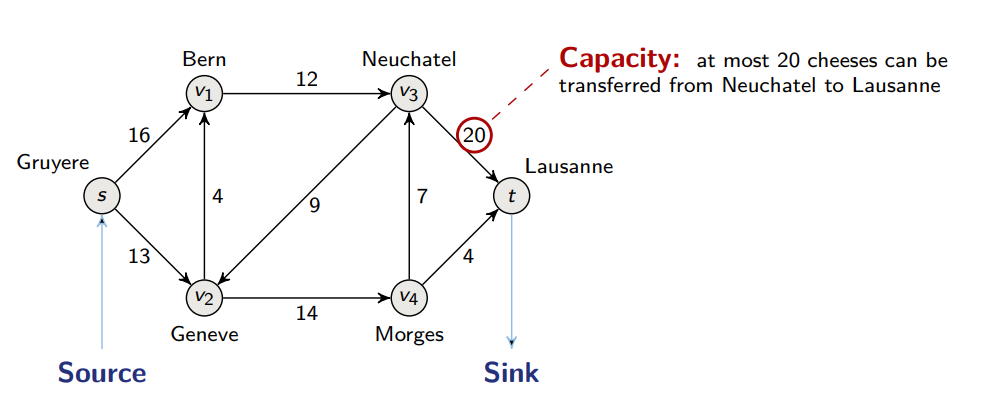
\includegraphics[width=\linewidth]{images/flow_network.png}
\end{center}

\begin{defn}[title=Formally]
\begin{itemize}
    \item Source: $s\in V$, sink: $t\in V$
    \item Directed graph (DG): $G=(V,E)$
    \item Each (u, v) has a capacity $c(u,v) \ge 0$
    \item No antiparallel: if $(u,v)\in E$, then $(v,u)\not\in E$
\end{itemize}
\end{defn}

\begin{thm}[title=Capacity constraint]
$\forall u,v\in V$, $0\le f(u,v)\le c(u,v)$
\end{thm}
\begin{thm}[title=Flow conservation]
$\forall u\in V\setminus\{s,t\}$,
$\sum_{v\in V} f(u,v) = \sum_{v\in V} f(v,u)$
\end{thm}

\begin{defn}[title=Cut]
Partition of $V$ into two disjoint sets $S$ and $T$ such that $s\in S$ and $t\in T$. $c(S,T)=\sum_{u\in S, v\in T} c(u,v)$.
\end{defn}

\subsection{Maximum flow problem - Ford-Fulkerson method}

\begin{prop}[title={Residual network $G_f=(V,E_f)$}]
$c_f(u,v)$: additional flow possible (forward edge) or removable (backward edge).
\end{prop}

\begin{lstlisting}
FORD-FULKERSON-METHOD(G, s, t)
    initialize flow f to 0
    while exists an augmenting path p in G_f
        b = bottleneck(p)
        augment flow along p by b
    return f
\end{lstlisting}

\subsection{Min cut problem}

\begin{defn}[title=Min cut]
It is a cut where the capacity crossing it is the minimum among all cuts.
\end{defn}

\begin{prop}[title=Net flow accross cut]
$f(S,T) = \sum_{u\in S, v\in T} f(u,v) - \sum_{u\in S, v\in T} f(v,u)$
\end{prop}

\begin{thm}[title=Max-flow min-cut theorem ($\Leftrightarrow$)]
\begin{itemize}
  \item f is the maximum flow
  \item $G_f$ has no augmenting path
  \item $|f| = c(S,T)$ for a minimum cut (S, T)
\end{itemize}
\end{thm}

\subsection{Applications of max flow}
\begin{prop}[title=Bipartite matching as flow]
$G=(V,E)$, $V=L\cup R$. Connect $s\to\forall u\in L$ and $\forall v\in R\to t$, all capacities 1. Run Ford-Fulkerson.
\end{prop}

\begin{prop}[title=Edge-disjoint paths]
Max \# edge-disjoint paths from $s$ to $t$ = min edges to remove to disconnect $s$ from $t$ = max flow (all capacities 1).
\end{prop}


% ============================================================
\section{Spanning Trees}

\begin{defn}[title=Definition]
Set $T$ of edges that is acyclic and spanning (connects all vertices of $G$).
\textbf{Goal of MST problem: }Find a spanning tree of min total weight.
\end{defn}

\begin{thm}[title=Cut property (safe edge)]
Given any cut, a minimum-weight crossing edge belongs to some MST.
\end{thm}

\subsection{Prim's algorithm}
\begin{lstlisting}
PRIM(G, w, r)    // G undirected ; w: E -> R weights
    Q = {}          // min-priority queue (min-heap)
    for each u in G.V:
        u.key = inf
        u.pi = NIL             // u.pi = parent in T
        INSERT(Q, u)
    DECREASE-KEY(Q, r, 0)               // r.key = 0
    while Q != {}:
        u = EXTRACT-MIN(Q)
        for each v in G.Adj[u]:
            if v in Q and w(u,v) < v.key:
                v.pi = u
                DECREASE-KEY(Q, v, w(u,v))
\end{lstlisting}

\begin{thm}[title=Why does it work?]
T is always a subtree of a MST.
\end{thm}

\begin{prop}[title=Prim's runtime]
$O(E\lg V)$ with binary heap. $O(V\lg V+E)$ with Fibonacci heap.
\end{prop}

\subsection{Kruskal's algorithm}
\begin{lstlisting}
KRUSKAL(G, w)
    A = {}
    for v in G.V: MAKE-SET(v)
    sort G.E by w non-decreasing
    for (u, v) in G.E (sorted):
        if FIND(u) != FIND(v)
            A += {(u,v)}; UNION(u, v)
    return A
\end{lstlisting}

\begin{thm}[title=Why does it work?]
T is always a sub-forest of a MST.
\end{thm}

\begin{prop}[title=Kruskal's runtime]
$O(E\lg E) = O(E\lg V)$ (sorting dominates).
\end{prop}

\newpage
% ============================================================
% The next part is autogenerated, needs to be checked

\section{Shortest Paths}

\begin{defn}[title=Problem variants]
\begin{itemize}
  \item \kv{Single-source}{from $s$ to all vertices}
  \item \kv{Single-dest.}{reverse edges $\to$ single-source}
  \item \kv{Single-pair}{no better w.c.\ than single-source}
  \item \kv{All-pairs}{solve single-source for each vertex}
\end{itemize}
\end{defn}

\begin{warn}[title=Negative weights]
Allowed if no negative-weight cycle is reachable from $s$. Dijkstra requires $w\geq 0$.
\end{warn}

\begin{prop}[title=Optimal substructure]
Any subpath of a shortest path is itself a shortest path (proof by contradiction).
\end{prop}

\begin{lstlisting}
INIT-SINGLE-SOURCE(G, s)
    for v in G.V: v.d = inf; v.pi = NIL
    s.d = 0

RELAX(u, v, w)
    if v.d > u.d + w(u, v)
        v.d = u.d + w(u, v); v.pi = u
\end{lstlisting}

\subsection{Bellman-Ford}

\begin{lstlisting}
BELLMAN-FORD(G, w, s)
    INIT-SINGLE-SOURCE(G, s)
    for i = 1 to |G.V| - 1
        for (u, v) in G.E: RELAX(u, v, w)
    for (u, v) in G.E        // neg-cycle check
        if v.d > u.d + w(u, v): return FALSE
    return TRUE
\end{lstlisting}

\begin{thm}[title=Correctness]
No neg-cycle reachable from $s$ $\Rightarrow$ after $|V|\!-\!1$ iterations, $v.d = \delta(s,v)$ $\forall v$. Shortest path uses $\leq |V|\!-\!1$ edges (can always remove cycle if non-negative weight).
\end{thm}

\begin{prop}[title=Negative cycle detection]
Neg-cycle reachable from $s$ $\Leftrightarrow$ some $\ell$-value changes in the $n$-th (extra) iteration.\\
\textbf{Proof:} If no change, $\forall(u,v)\in E: \ell(u)+w(u,v)\geq\ell(v)$. Summing over any cycle gives $\sum w(v_{i-1},v_i)\geq 0$.
\end{prop}

\begin{prop}[title=Runtime]
$\Theta(E\cdot V)$. Good for distributed routing: each vertex repeatedly asks neighbors for best path.
\end{prop}

\subsection{Dijkstra's Algorithm}
Non-negative weights only. Greedy (essentially weighted BFS, like Prim's).

\begin{lstlisting}
DIJKSTRA(G, w, s)
    INIT-SINGLE-SOURCE(G, s)
    Q = G.V   // min-heap on d
    while Q != {}:
        u = EXTRACT-MIN(Q)
        for v in G.Adj[u]: RELAX(u, v, w)
\end{lstlisting}

\begin{prop}[title=Runtime]
$O(E\lg V)$ with binary heap. $O(V\lg V+E)$ with Fibonacci heap.
\end{prop}

% ============================================================
\section{Probabilistic Analysis}

\subsection{Motivation}
Worst case rarely happens. Randomization helps avoid worst-case and adversarial inputs (e.g., random pivot in quicksort). Also necessary in cryptography.

\subsection{Indicator Random Variables}

\begin{defn}[title=Indicator RV]
Given sample space and event $A$:
\[I\{A\} = \begin{cases}1 & A\text{ occurs}\\0 & \text{otherwise}\end{cases}\]
\textbf{Lemma:} $\E[I\{A\}] = \Pr\{A\}$\quad (since $\E[X_A]=1\cdot\Pr\{A\}+0\cdot\Pr\{\bar{A}\}$)
\end{defn}

\begin{thm}[title=Linearity of expectation]
$\E[aX+bY] = a\E[X]+b\E[Y]$\\
\emph{Holds even when $X$ and $Y$ are dependent!}
\end{thm}

\subsection{Hiring Problem}
Hire candidate if taller than current best; $n$ candidates, random arrival order.
\begin{itemize}
  \item Worst case: $n$ hires (candidates arrive sorted)
  \item Let $X_i = I\{\text{candidate }i\text{ hired}\}$, $X = \sum_{i=1}^n X_i$
  \item $\Pr\{\text{candidate }i\text{ hired}\} = \frac{1}{i}$ (is tallest among first $i$)
  \item By linearity: $\E[\#\text{hires}] = \sum_{i=1}^{n}\frac{1}{i} = H_n = \ln n + O(1)$
\end{itemize}
Expected number of hires is $O(\ln n)$ vs worst case $O(n)$.

% ============================================================
\section{Hash Tables}

\begin{defn}[title=Hash function]
$h: U\to\{0,\ldots,m{-}1\}$ maps key universe to $m$ slots.\\
\textbf{Collision:} $h(k_1)=h(k_2)$ with $k_1\neq k_2$.\\
\textbf{Load factor:} $\alpha = n/m$ (number of keys / slots).
\end{defn}

\begin{prop}[title=Chaining (collision resolution)]
Each slot: linked list of keys. Insert $O(1)$. Search/Delete $\Theta(1{+}\alpha)$ average. If $n=O(m)$ then $\alpha=O(1)$: all ops $O(1)$.
\end{prop}

\begin{prop}[title=Division method]
$h(k) = k \bmod m$. Avoid $m=2^p$ (only uses low-order bits of $k$).
\end{prop}

\begin{prop}[title=Multiplication method]
$h(k) = \lfloor m\cdot(kA \bmod 1)\rfloor$,\quad $0 < A < 1$.
\end{prop}

\begin{prop}[title=Birthday paradox]
$n$ items into $m$ slots: collision likely when $n\gtrsim\sqrt{2m}$.\\
$\Pr[\text{collision}]\geq\tfrac{1}{2}$ when $n\geq\sqrt{2m\ln 2}\approx 1.18\sqrt{m}$.
\end{prop}

\begin{prop}[title=Birthday lemma]
Prob.\ of \emph{no} collision among $q$ items drawn uniformly from $[n]$:
$\leq e^{-q(q-1)/(2n)}$.
\end{prop}

\end{multicols*}
\end{document}
